\section{Conclusioni}

Siamo riusciti ad analizzare in modo accurato un filtro passa basso, ottenendo valori sperimentali compatibili con la legge teorica ricavata dalla risoluzione.

\begin{wrapfigure}[33]{r}[0pt]{115mm}
%	\centering
    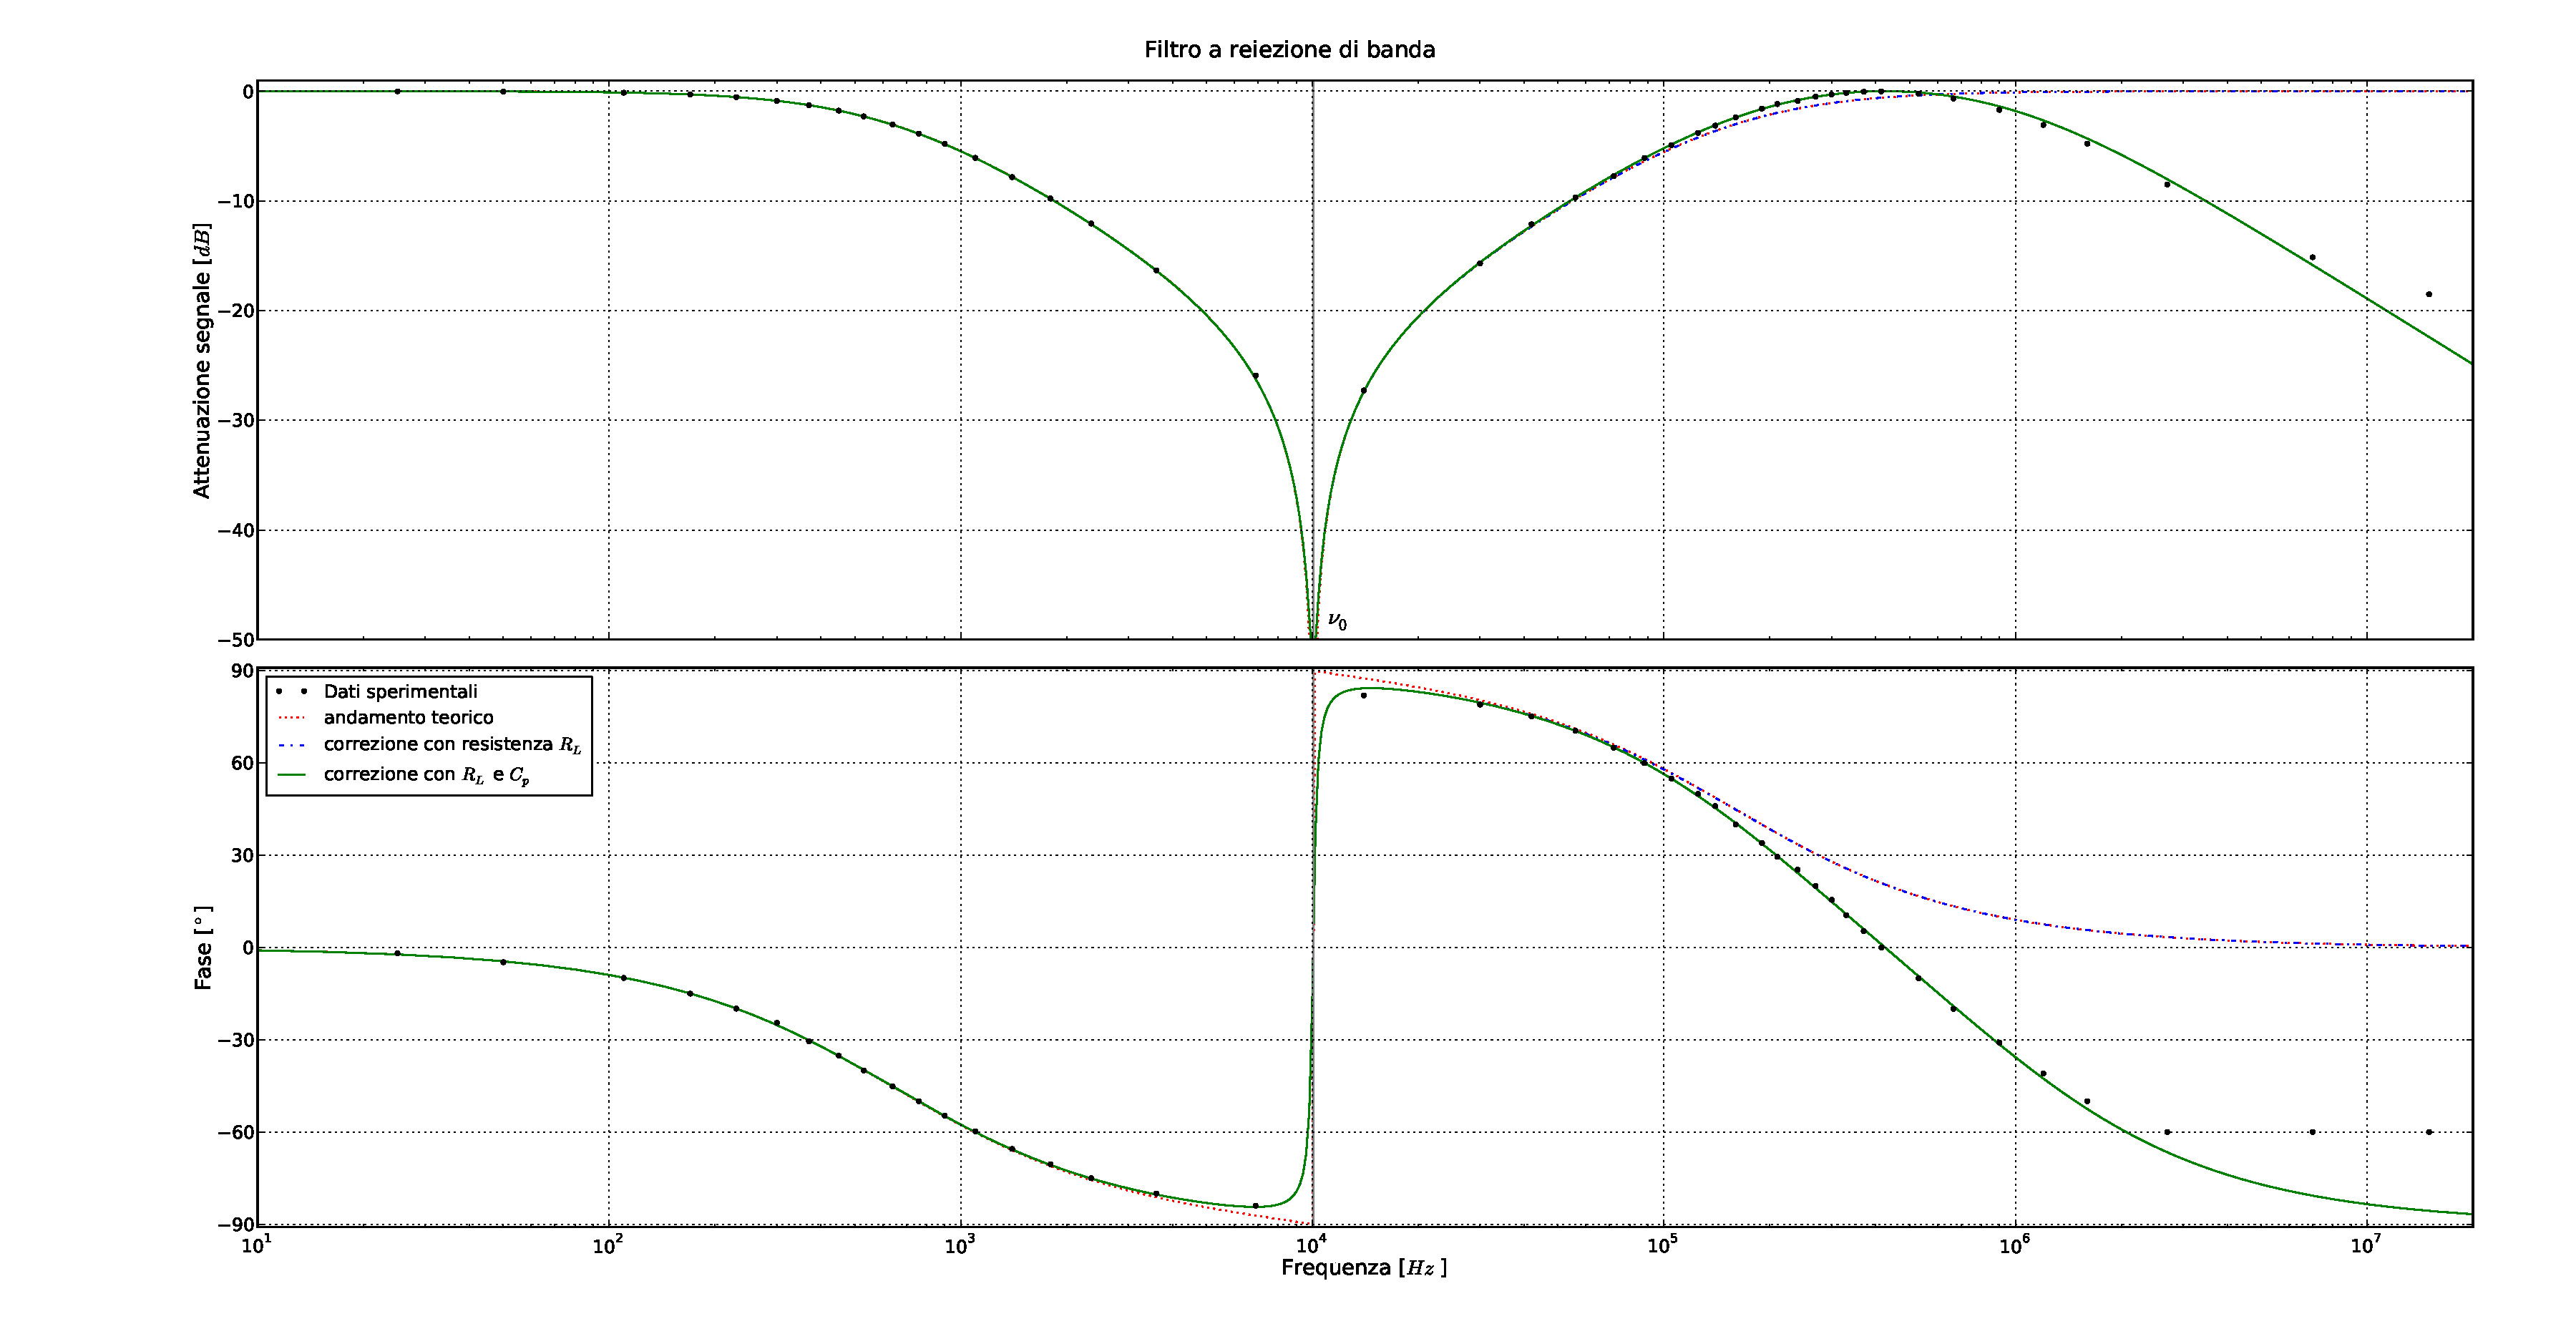
\includegraphics[width=120mm]{notch.pdf}
    \caption{Diagrammi di Bode per il filtro a reiezione di banda.}
    \label{fig:notch}
\end{wrapfigure}

Non possiamo invece dire lo stesso per gli altri due tipi di filtri. Infatti non è stato possibile usare le leggi teoriche ricavate dallo studio circuitale ma si è rivelato necessario apportare delle modifiche (aggiunta di elementi) per ottenere leggi compatibili con i dati sperimentali. Il motivo per cui il modello teorico non approssima bene i dati reali è essenzialmente il fatto che condensatori, resistenze, induttanze e cavi non sono ideali. Nel caso del passa basso non si è vista questa incongruenza forse perchè il circuito utilizzato era estremamente semplice. 

Non siamo riusciti a capire il motivo per cui i dati relativi al filtro passa banda si discostano sulle code dalla legge anche se corretta con $R_L$. Infatti, osservando il grafico della fase, si nota immediatamente come la correzione sia stata efficace.

Il filtro che più si è rivelato complicato nell'analisi è stato quello a reiezione di banda. Sebbene sia stata applicata quasi subito la correzione già utilizzata nell'analisi del filtro passa banda (inserimento di una resistenza $R_L$), per le alte frequenze ($>10^5 \si{\hertz}$) si è comunque avuta un'enorme discrepanza con i dati sperimentali. Ciò che più ci ha fatto riflettere è stato il fatto che sia fase che intensità del segnale in $output$ erano incompatibili. Infatti, nel caso del filtro passa banda, solo l'intensità del segnale in uscita non era compatibile con la previsione, mentre la fase lo era. Ciò lascia credere ci sia un errore nella stima di differenza di potenziale picco-picco, ma non nella legge teorica. Nel caso del filtro a reiezione di banda, invece, l'incompatibilità sia dell'intensità del segnale sia della fase fa sicuramente pensare ad un errore nella legge trovata. Abbiamo dunque cercato di perfezionare il nostro modello, giungendo a due ipotesi.

Come prima ipotesi abbiamo considerato le induttanze parassite $R_p$ dei fili (ogni filo ho una propria induttanza). Abbiamo risolto nuovamente il circuito aggiungendo un'induttanza in serie subito prima della resistenza $R$ e poi, eseguendo vari plot per diversi valori di $R_p$, ne abbiamo analizzato l'andamento. Anche in questo caso l'analisi ha dato esito negativo. Tale correzione non ha purtroppo portato un miglioramento nella compatibilità con i dati da noi raccolti.

Come seconda ipotesi si è pensato a qualche tipo di capacità parassita $C_p$. Infatti, dall'andamento dei dati si vede uno smorzamento per alte frequenze. Si è dunque provato ad aggiungere una capacità in parallelo all'induttanza, così da isolare l'induttanza per alte frequenze. Risolvendo nuovamente il circuito si è visto che tale scelta, per determinati valori di $C_p$, era compatibile con i dati sperimentali. Si è stimato graficamente che per un valore di $C_p \approx 140 \si{\pico\farad}$ sia il grafico della fase sia quello dell'intensità di segnale risultano corretti. Nonostante ciò, gli ultimi 3 dati, come si può notare in Fig.$\,$\ref{fig:notch}, si discostano comunque di molto dalla legge. Ciò è probabilmente da ricondurre al fatto che le frequenze erano molto alte ($\approx 10 \si{\mega\hertz}$) e pertanto l'oscilloscopio e in particolar modo il generatore di forme d'onda, la cui frequenza massima è \SI{15}{\mega\hertz}, erano al limite delle loro possibilità.






%l'\emph{effetto pelle}. Tale fenomeno si presenta in maniera visibile per lo più ad alte frequenze e consiste nel fatto che la corrente tende a scorrere con più facilità sulla superficie del conduttore (ricordiamo che in regime quasi stazionario la corrente scorre uniformemente all'interno di un conduttore omogeneo e isotropo) che al centro del conduttore. Tale effetto potrebbe causare una capacità parassita. Tuttavia, provando ad aggiungere condensatori in serie al circuito, abbiamo visto subito che essi non causerebbero modifiche nella legge teorica per alte frequenze. Abbiamo dunque escluso l'effetto pelle.

%Non sappiamo dunque ancora quale sia la causa di tale discrepanza. 